\section{Supporting Information: PDIpy}

\begin{figure}
    \centering
    \begin{tabular}{c|c}
        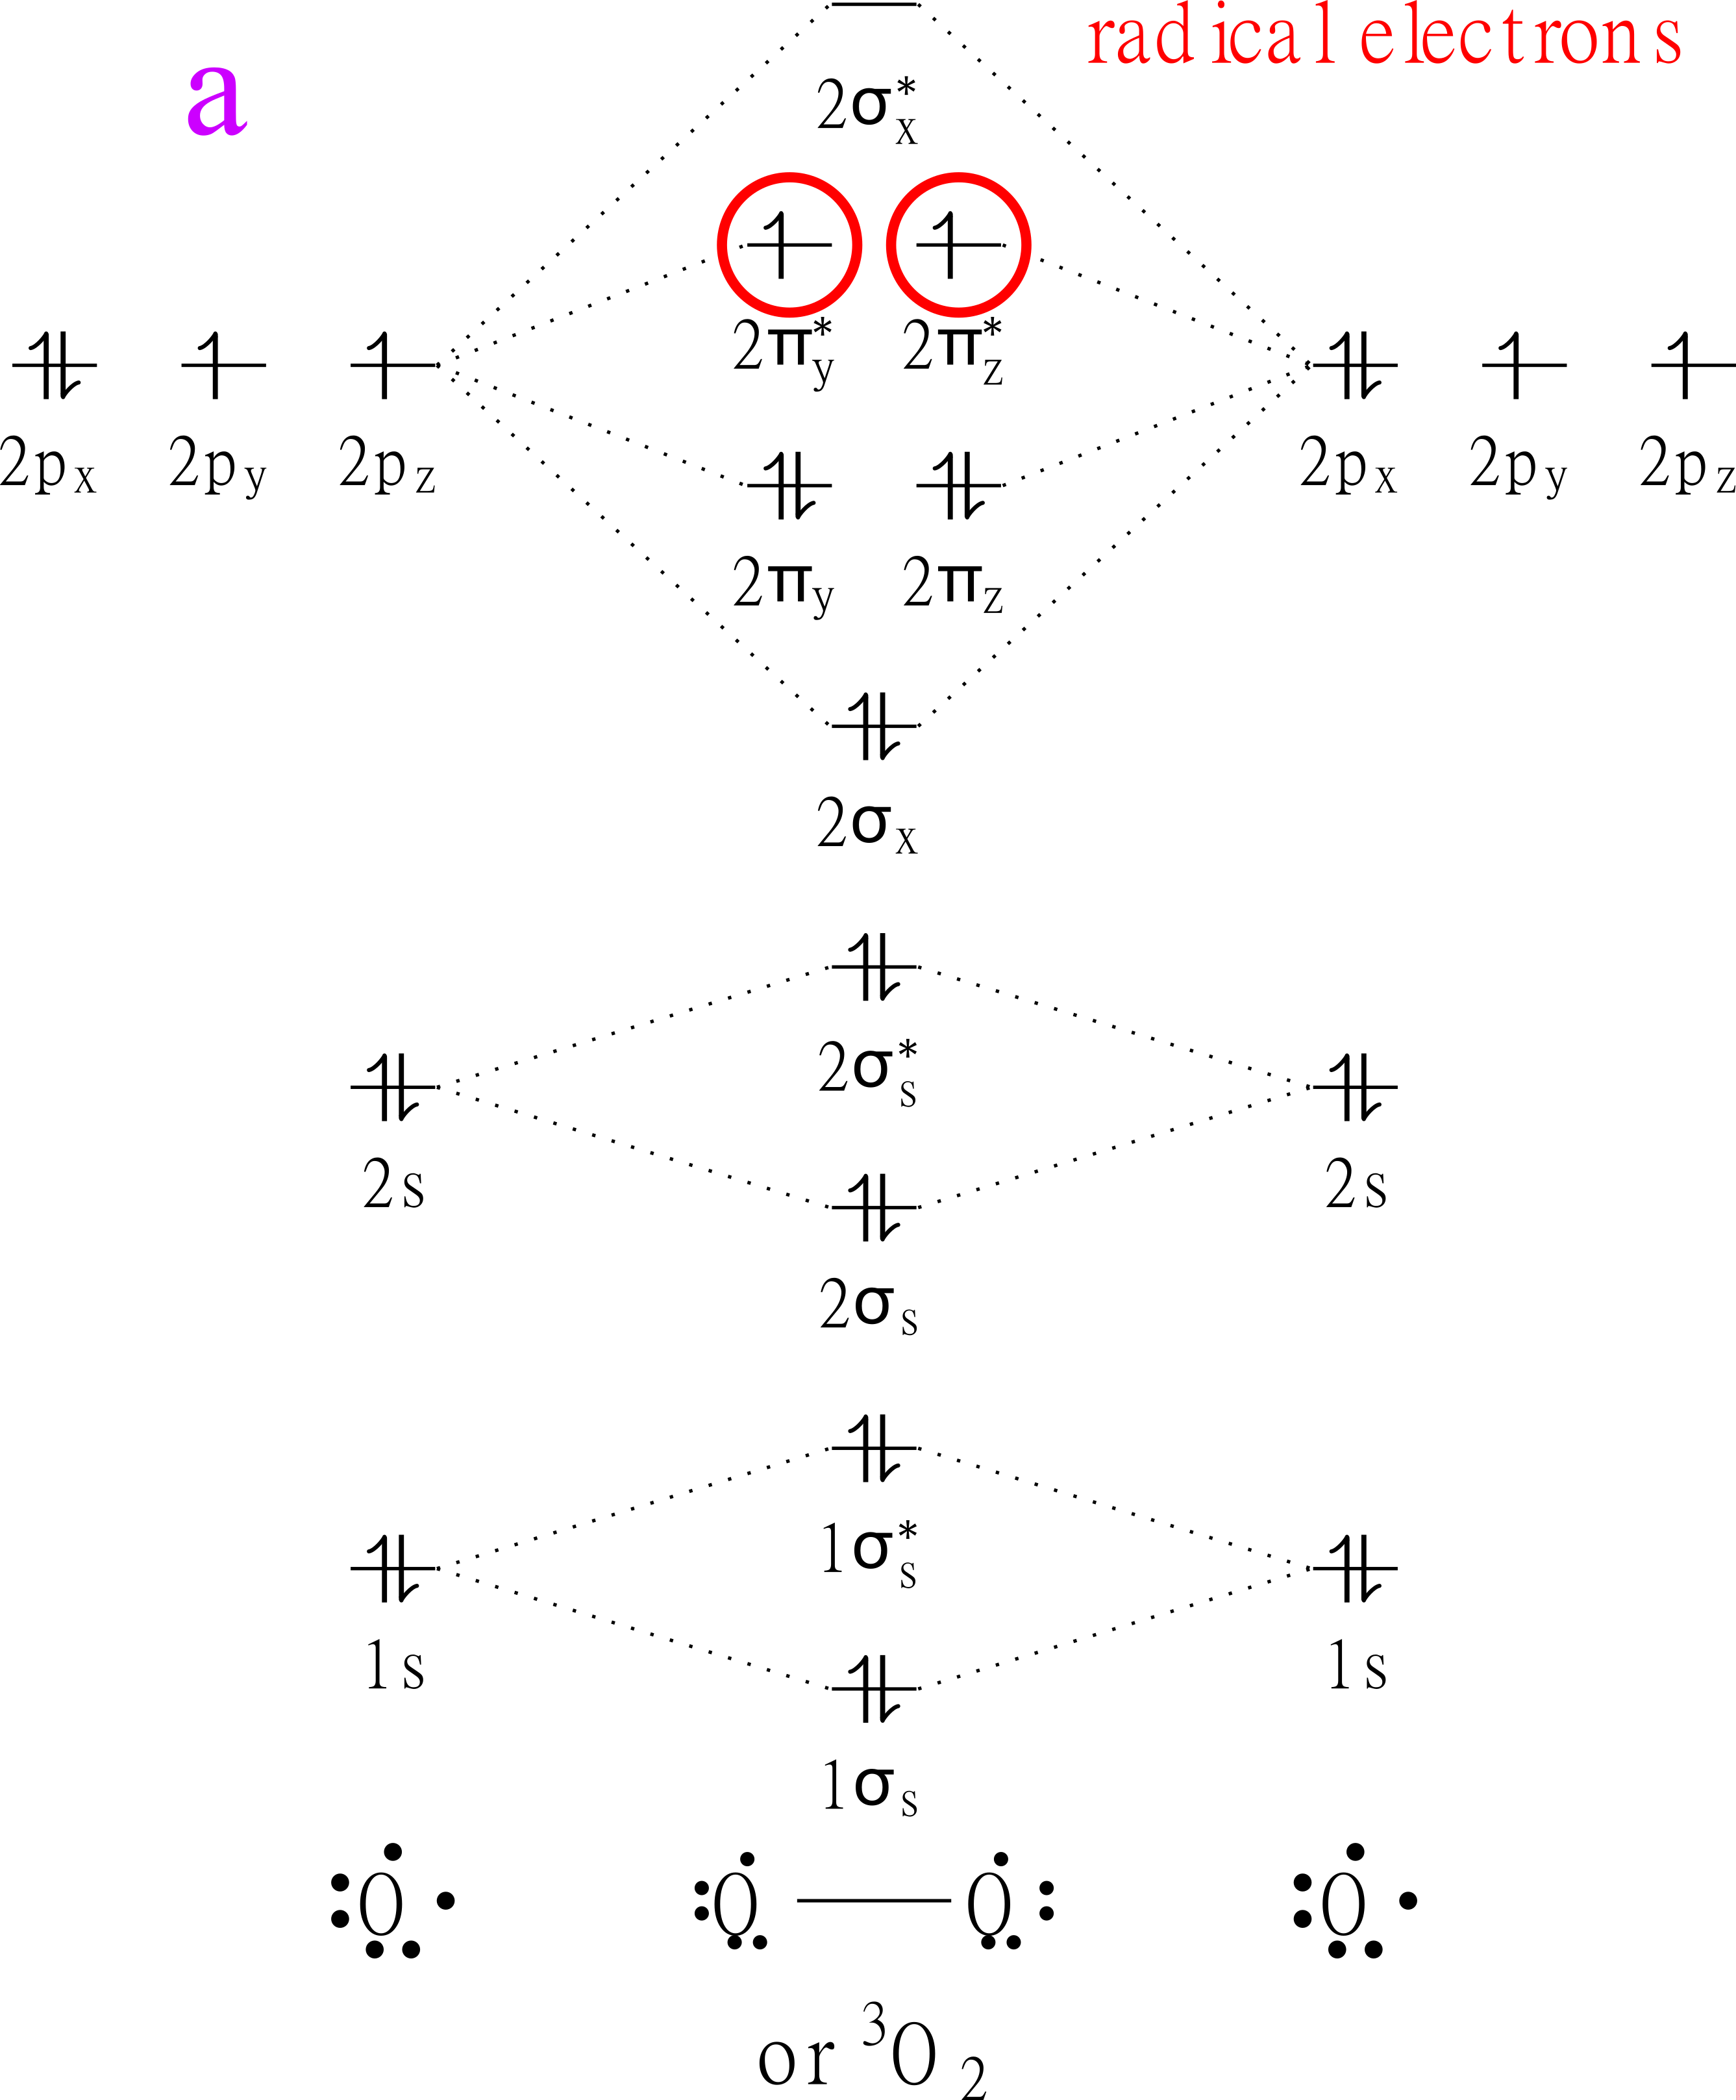
\includegraphics[width = 0.48\textwidth]{images/PDIpy/triplet_mo_diagram.png}
        & 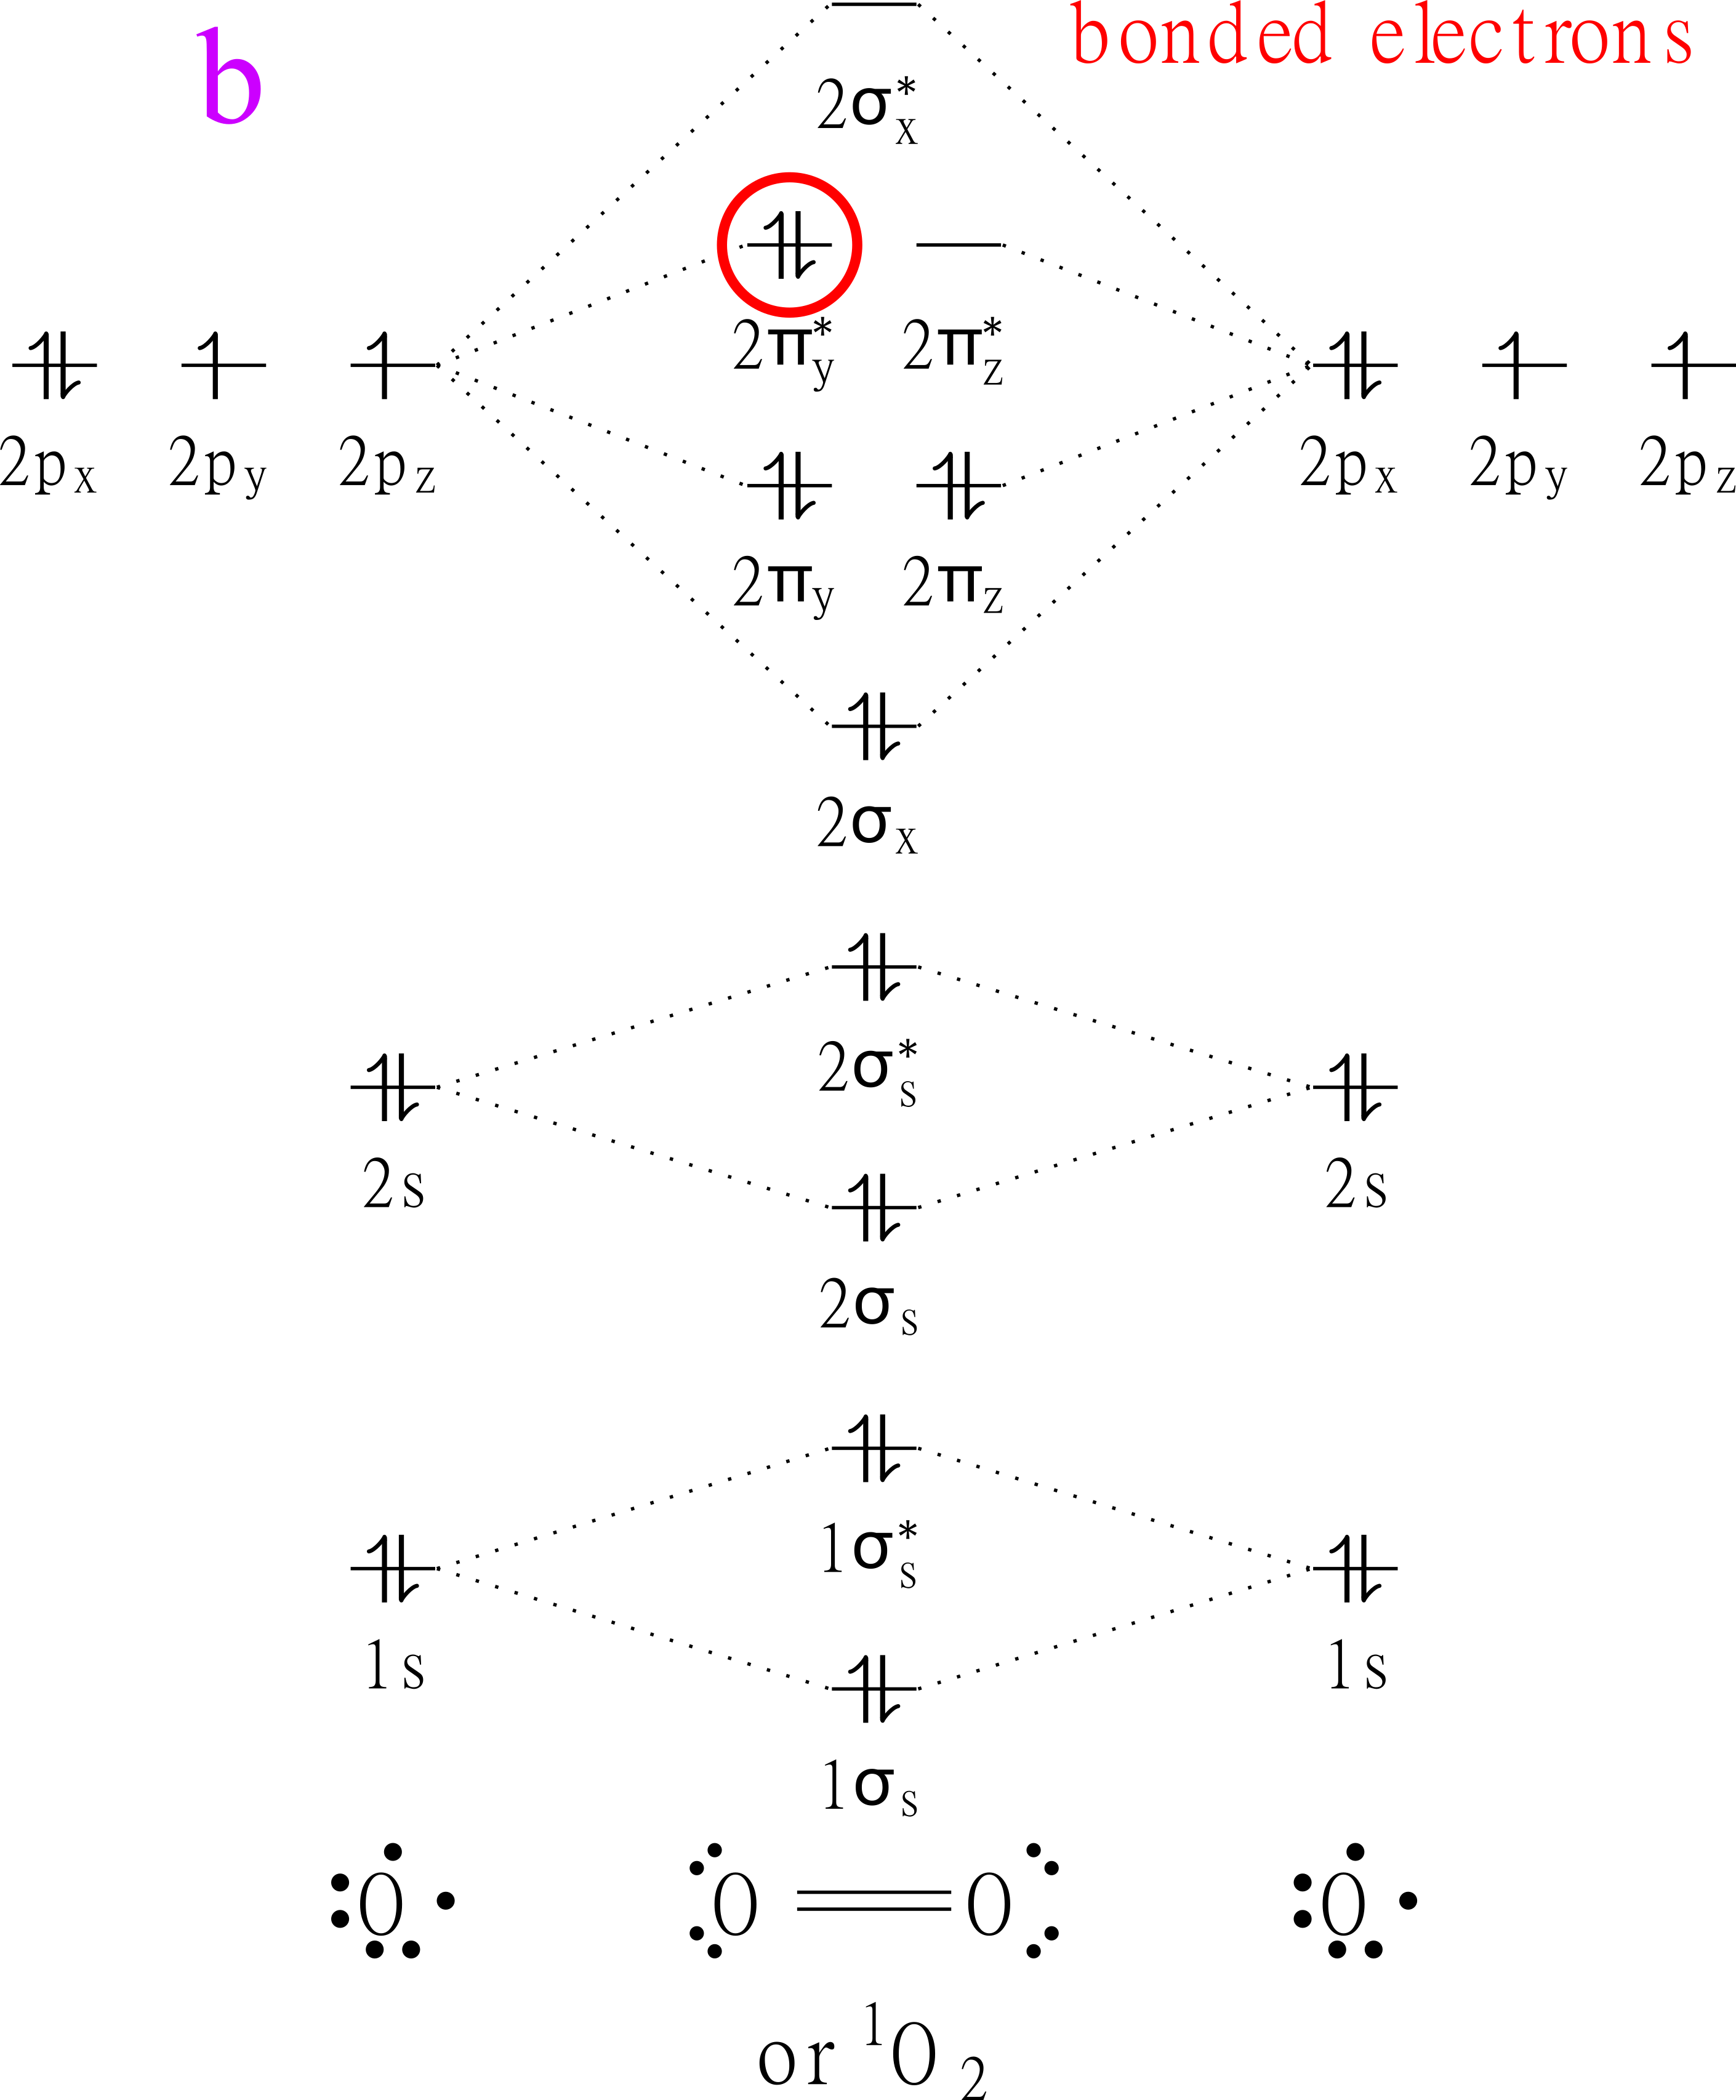
\includegraphics[width = 0.48\textwidth]{images/PDIpy/singlet_mo_diagram.png} \\
    \end{tabular}
    \caption{
        Qualitative orbital diagrams for diatomic oxygen. Each barbed arrows represent single electron, and each platform represents the electronic orbital of the respective label. Panel a) depicts the ground triplet state ($\ce{^3O2^.}$), which characteristically contains two radical electrons in its highest occupied molecular orbital (HOMO). Panel b) depicts the excited singlet state ($\ce{^1O2}$), which characteristically contains a $\pi^*$-bond in its HOMO that destabilizes the molecule and contributes to greater reactivity.
    }
    \label{mo_diagrams}
\end{figure}


% \subsection*{Oxidized membrane proportions}
% The proportion of bacterial fatty acids that are oxidized by singlet oxygen is a proxy for cellular killing and thus reduction of the bacterial population. The bacterial cell radius $radius_{cell, outer}$ can be calculated from its volume $volume_{cell}$
% \begin{equation}
%     radius_{cell, outer} = \sqrt[3]{3*\frac{volume_{cell}}{4\pi}}
% \end{equation}
% which is often reported in literature. The volume of the membrane 
% \begin{equation}
%     volume_{membrane} = \frac{4\pi}{3}*(radius_{cell,outer}^3 - radius_{cell,inner}^3)
% \end{equation}
% can be calculated as the difference between the inner $radius_{cell, inner}$ and outer cell radii. The area of the membrane that is oxidized can be quantified
% \begin{equation}
%     area_{oxidized} = 2\pi * radius_{cell, outer}^2 * (1-angle_{oxidation})
% \end{equation}
% and compared to the total membrane area of the cell
% \begin{equation}
%     area_{membrane} = \pi * radius_{cell, outer}^2
% \end{equation}
% in a ratio of oxidized membrane
% \begin{equation} \label{oxidation_scalar}
%     scalar_{oxidized} = \frac{area_{oxidized}}{area_{membrane}}
% \end{equation}
% that signifies the proportion of oxidation. The scalar from \cref{oxidation_scalar} is applied to the chemical concentrations to accurately reflect the extent of oxidation in the afflicted portion of the membrane during PDI treatment. A scalar can similarly be derived from a ratio of volumes, where the volume of the oxidized cap
% \begin{equation}
%     volume_{oxidized} = \frac{2\pi}{3}*(1-angle_{oxidized})\\ 
%         *(radius_{cell,outer}^3 - radius_{cell,inner}^3)    
% \end{equation}
% and the $volume_{membrane}$ an be arranged in a quotient 
% \begin{equation}
%     scalar_{oxidized} = volume_{oxidized} / volume_{membrane} 
% \end{equation}
% for the oxidation quotient. 
